\documentclass{beamer}
\usepackage{hyperref}
\usepackage[T1]{fontenc}
\usepackage{cite}
\usepackage{relsize}
\usepackage{animate}


\usefonttheme[onlymath]{serif}
%C++ symbol
\newcommand{\Rplus}{\protect\hspace{-.1em}\protect\raisebox{.35ex}{\smaller{\smaller\textbf{+}}}}
\newcommand{\Cpp}{\mbox{C\Rplus\Rplus}\hspace{3pt}}
%Scientific notation
\newcommand{\expnumber}[2]{{#1}\mathrm{e}{#2}}

\usepackage{latexsym,amsmath,xcolor,multicol,booktabs,calligra}
\usepackage{graphicx,tikz,listings,stackengine}
\usetikzlibrary{shapes,snakes,matrix, positioning,arrows.meta}
\setbeamertemplate{bibliography item}[text]

\author{Rafael De Luna Loredo}
\title{Programaci\'on en Python y \Cpp}
\subtitle{Arreglos y Matrices}
\institute{Facultad de Ciencias, UASLP}
\date{}
\usepackage{NJFU}

% defs
\def\cmd#1{\texttt{\color{red}\footnotesize $\backslash$#1}}
\def\env#1{\texttt{\color{blue}\footnotesize #1}}
\definecolor{deepblue}{rgb}{0,0,0.5}
\definecolor{deepred}{rgb}{0.6,0,0}
\definecolor{deepgreen}{rgb}{0,0.5,0}
\definecolor{halfgray}{gray}{0.55}

\begin{document}
	
	\AtBeginSubsection[]
	{
		\begin{frame}
			\begin{multicols}{3}
				\tableofcontents[currentsection,subsectionstyle=show/shaded/hide,subsubsectionstyle=show/shaded/hide]
			\end{multicols}
		\end{frame}
	}
	\AtBeginSubsubsection[]{
		\begin{frame}
			\begin{multicols}{3}
				\tableofcontents[currentsection,subsectionstyle=show/shaded/hide,subsubsectionstyle=show/shaded/hide]
			\end{multicols}
		\end{frame}
	}
	
	\AtBeginSection[]
	{
		\begin{frame}
			\begin{multicols*}{3}
				\tableofcontents[currentsection,subsectionstyle=show/shaded/hide,subsubsectionstyle=show/shaded/hide]
			\end{multicols*}
		\end{frame}
	}
	
	\begin{frame}
		\titlepage
		\begin{figure}[htpb]
			\begin{center}
				
\includegraphics[width=0.2\linewidth]{fig/logo.png}
			\end{center}
		\end{figure}
	\end{frame}
	
	\begin{frame}{Indice}
		\begin{multicols*}{3}
			\tableofcontents[sectionstyle=show,subsectionstyle=show/shaded/hide,subsubsectionstyle=show/shaded/hide]
		\end{multicols*}
	\end{frame}

\section{Arreglos}
\begin{frame}{\textquestiondown Qu'e son?}
	\begin{itemize}
		\item Podemos considerarlos una estructura de datos de un solo tipo
		\item Puede contener m\'ultiples valores
		\item Es unidimensional
		\item Su espacio en memoria var\'ia seg\'un el tipo de dato y los valores que pueda tener
		\item En Python como tal no existen,  se usan las listas en su lugar
		\item El \'indice siempre empieza en cero, puede variar en algunos lenguajes.
	\end{itemize}
\end{frame}


\begin{frame}{Almacenamiento en memoria}
	\begin{itemize}
		\item El valor nos \'indica el contenido del arreglo en determinada posici\'on
		\item El \'indice nos indica la posici\'on en el arreglo
		\item La direcci\'on de memoria donde se encuentra almacenado dicho valor	
	\end{itemize}
	\centering
	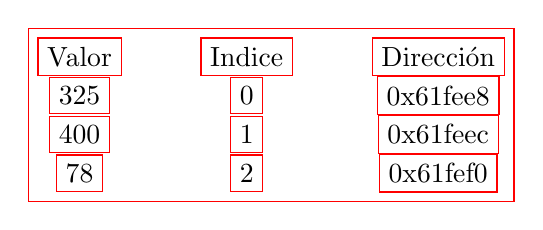
\begin{tikzpicture}[ampersand replacement=\&,every node/.style={draw}]
		\matrix [draw=red,column sep=1cm]
		{
			\node {Valor}; \& \node {Indice}; \& \node{Direcci\'on}; \\
			\node {325}; \& \node{0}; \& \node {0x61fee8}; \\
			\node {400}; \& \node{1}; \& \node {0x61feec}; \\
			\node {78}; \& \node{2}; \& \node {0x61fef0}; \\
		};
	\end{tikzpicture}
\end{frame}

\subsection{M\'etodos}

\begin{frame}{Insertar en \Cpp}
	\begin{itemize}
		\item Hay que conocer el \'indice donde queremos el valor
		\item No es necesario insertarlos en orden
		\item No se puede tener un \'indice mayor al tamaño del arreglo
	\end{itemize}
	\centering
	\animategraphics[autoplay,loop,width=4cm]{20}{animaciones/array/insertion/insertion-}{0}{216}
\end{frame}

\begin{frame}{Insertar en Python}
	\begin{itemize}
		\item Las listas en Python tienen un m\'etodo para agregar valores
		\item No es necesario conocer el \'indice
		\item No es necesario conocer el tamaño 
	\end{itemize}
\end{frame}

\begin{frame}{Modificar}
	\begin{itemize}
		\item Hay que conocer el \'indice
		\item No se puede tener un \'indice mayor al tamaño del arreglo
	\end{itemize}
\end{frame}

\begin{frame}{Eliminar}
	\begin{itemize}
		\item En \Cpp no se puede eliminar un elemento de un arreglo, solo se ignora el \'indice 
		\item En Python existen 3 m\'etodos \footnote{Si se elimina un elemento, el tamaño y los \'indices cambian}
		\begin{itemize}
			\item Por el \'ultimo \'indice
			\item Por \'indice
			\item Por valor
		\end{itemize}
		\animategraphics[autoplay,loop,width=3cm]{20}{animaciones/array/elimination/elimination-}{0}{194}
		\animategraphics[autoplay,loop,width=3cm]{20}{"animaciones/array/elimination_value/"elimination_value-}{0}{149}
		\animategraphics[autoplay,loop,width=3cm]{20}{animaciones/array/drop/drop-}{0}{194}
	\end{itemize}
\end{frame}

\section{Matrices}
\begin{frame}{Introducci\'on}
	\begin{itemize}
		\item Son de un solo tipo
		\item Puede contener m\'ultiples valores
		\item Son bidimensionales
		\item Su espacio en memoria var\'ia seg\'un el tipo de dato y los valores que pueda tener
		\item En Python como tal no existen, se usan listas que contienen listas
		\item El \'indice siempre empieza en cero, puede variar en algunos lenguajes, pero suele ser una regla general
		\item Tienen doble índice, uno para las filas y otro para las columnas
		\item Las filas y columnas no tienen que ser del mismo tamaño
	\end{itemize}
\end{frame}

\subsection{M\'etodos}
\begin{frame}{Insertar en \Cpp}
	\begin{itemize}
		\item Hay que conocer ambos indices donde queremos agregar el valor
		\item No es necesario insertarlos en orden
		\item No se pueden tener indices mayores a las filas o columnas
	\end{itemize}
	\centering
	\animategraphics[autoplay,loop,width=4cm]{50}{animaciones/matrices/insertion/insertion-}{0}{440}
\end{frame}

\begin{frame}{Insertar en Python}
	\begin{itemize}
		\item Hay que conocer los indices donde se ubican las listas
		\item No es necesario conocer el \'indice
		\item No es necesario conocer el tamaño 
	\end{itemize}
\end{frame}

\begin{frame}{Modificar}
	\begin{itemize}
		\item Hay que conocer el \'indice
		\item No se puede tener un \'indice mayor al tamaño del arreglo
	\end{itemize}
\end{frame}

\begin{frame}{Eliminar}
	\begin{itemize}
		\item En \Cpp no se puede eliminar un elemento de una matriz, solo se ignora el \'indice 
		\item En Python
		\begin{itemize}
			\item Por el \'ultimo \'indice
			\item Por \'indice
			\item Por valor \nocite{BHASIN,BJARNE1,BJARNE2,CAIRO,CPP,DEITEL,DOWNEY,JAWORSKI,KENN,lAAKMANN,MATTHES,RAMALHO,SED,BRASSARD}
		\end{itemize}
		\animategraphics[autoplay,loop,width=3cm]{20}{animaciones/matrices/elimination/elimination-}{0}{239}
		\animategraphics[autoplay,loop,width=3cm]{20}{"animaciones/matrices/elimination_value/elimination_value-"}{0}{233}
		\animategraphics[autoplay,loop,width=3cm]{20}{animaciones/Matrices/drop/drop-}{0}{254}
	\end{itemize}
\end{frame}

\section{Referencias}
\subsection{}
\begin{frame}[allowframebreaks]
	
	\frametitle{Referencias}
	\bibliographystyle{acm}
	\bibliography{ref.bib}
\end{frame}

\end{document}